% Use only LaTeX2e, calling the article.cls class and 12-point type.

\author{H. Mostafavi, A. Harpak, D. Conley, J.K. Pritchard, M. Przeworski}
\documentclass[hidelinks, 12pt]{article}
%\usepackage{scicite}
\usepackage{times}
\topmargin 0.0cm
\oddsidemargin 0.2cm
\textwidth 16cm 
\textheight 21cm
\footskip 1.0cm
\newenvironment{sciabstract}{%
\begin{quote} \bf}
{\end{quote}}


%\usepackage{amsmath}% http://ctan.org/pkg/amsmath
%\usepackage{kbordermatrix}% http://www.hss.caltech.edu/~kcb/TeX/kbordermatrix.sty
\usepackage{bm}
\usepackage{mathtools}
\usepackage{blkarray, bigstrut} %
\usepackage{hyperref}
\usepackage{graphicx}
\usepackage{pdfpages}
\usepackage{chngcntr}
%\counterwithin{figure}{section} 
\usepackage{geometry}
\usepackage{caption}
\usepackage{subcaption}
%\usepackage{csvsimple}
\usepackage{pgfplotstable}
\usepackage[strict]{changepage}
% recommended:
\usepackage{booktabs}
\usepackage{array}
\usepackage{colortbl}
\usepackage{longtable}

%\usepackage[]{nohyperref}  % This makes hyperref commands do nothing without errors
%\usepackage{url}

\usepackage[utf8]{inputenc}
\usepackage{fullpage}%, palatino}
\usepackage{setspace}
\usepackage{helvet}
\usepackage{amsmath,amssymb}
%\doublespacing
\usepackage{color,soul}
%\usepackage{natbib}
\usepackage{titlesec}
\usepackage{bbm}
\usepackage{kbordermatrix}% http://www.hss.caltech.edu/~kcb/LaTeX.shtml
\usepackage{mathtools}
\usepackage{amsmath}




% The following lines set up an environment for the last note in the
% reference list, which commonly includes acknowledgments of funding,
% help, etc.  It's intended for users of BibTeX or the {thebibliography}
% environment.  Users who are hand-coding their references at the end
% using a list environment such as {enumerate} can simply add another
% item at the end, and it will be numbered automatically.

\newcounter{lastnote}
\newenvironment{scilastnote}{%
\setcounter{lastnote}{\value{enumiv}}%
\addtocounter{lastnote}{+1}%
\begin{list}%
{\arabic{lastnote}.}
{\setlength{\leftmargin}{.22in}}
{\setlength{\labelsep}{.5em}}}
{\end{list}}

\newcommand{\beginsupplement}{%
    \setcounter{table}{0}
    \renewcommand{\thetable}{S\arabic{table}}%
    \setcounter{figure}{0}
    \renewcommand{\thefigure}{S\arabic{figure}}%
}

%\captionsetup[sub]{format=plain,labelfont={sc,bf},labelformat=simple}
%\captionsetup[sub]{format=plain,labelfont={sc}}
%\captionsetup{labelfont={sf,up}, labelsep=period, format = plain, singlelinecheck = false}
\captionsetup[subfloat]{labelfont = {up},format = plain,labelformat = simple, labelsep = period}
\renewcommand{\thesubfigure}{\Alph{subfigure}}
% Include your paper's title here

\title{Poor portability of polygenic scores even within an ancestry group} 


% Place the author information here.  Please hand-code the contact
% information and notecalls; do *not* use \footnote commands.  Let the
% author contact information appear immediately below the author names
% as shown.  We would also prefer that you don't change the type-size
% settings shown here.

%\author
%{Xun Lan$^{1}$, anyone else?, Jonathan K. Pritchard$^{1,2, 3\ast}$\\
%\\
%\normalsize{$^{1}$Department of Genetics, Stanford University}\\
%\normalsize{$^{2}$Department of Biology, Stanford University}\\
%\normalsize{$^{3}$Howard Hughes Medical Institute, Stanford University}\\
%\\
%\normalsize{$^\ast$To whom correspondence should be addressed:  arbelh@stanford.edu.}
%}

% Include the date command, but leave its argument blank.




%%%%%%%%%%%%%%%%% END OF PREAMBLE %%%%%%%%%%%%%%%%




\begin{document} 
% Double-space the manuscript.
\baselineskip24pt
% Make the title.

\maketitle 
\begin{center}
\end{center}
\clearpage

\begingroup
  \hypersetup{hidelinks}
  \tableofcontents
\endgroup

\listoffigures
\listoftables

\pagebreak

\beginsupplement

\paragraph{Key implications}
ffdsafs

\section{Matching sib-regression and standard GWAS sample sizes}
We are looking for sample size $n^*$ of a standard GWAS using unrelated individuals such that if we use the estimated effects in a polygenic score, the prediction accuracy matches the prediction accuracy of a polygenic score based on a sib regression with sample size $n_{pairs}$. Throughout, we assume that all causal sites $i$ are known and unlinked, and that there is no population stratification or assortative mating.  We begin by finding the error associated with estimating the effect for a single site in each type of GWAS.  We will then examine (and match) the prediction accuracy of the polygenic scores composed from effects estimated in the unrelated/sib estimation sets, $\hat{\beta}_{ur},\hat{\beta}_{sib}$---on a new, independent prediction set $\{(x',y')\}$.

\subsection{Error of the estimated effect at a single site}
In the unrelated sample GWAS, our model is
$$y=g+e$$
where $e$ is the environmental effect (including all random noise) and
$$g=\beta^{ur}_0+\sum_{i}\beta_ix_i$$ 
is the polygenic score.  Our model for the effect of site $i$ is 
\begin{equation}
\label{ols_model}
y=\beta_0+\beta_ix_i+\epsilon_i,
\end{equation}
where 
$$\epsilon_i=g-\beta_i x_i+e,$$
with variance
$$Var[\epsilon_i]=Var[g-\beta_i x_i]+Var[e] = Var[y]-ֿ\beta_i^2Var[x_i].$$
In OLS regression for the effect of site $i$, the standard error is
$$Var[\hat{\beta}^{ur}_i]=\frac{Var[\epsilon_i]}{(n-1) Var[x_i^{ur}]} = \frac{Var[y]-ֿ\beta_i^2Var[x_i]}{(n-1)Var[x_i]},$$
where $n$ is the sample size.  In sib regression our model for site $i$ is
$$\Delta y=\beta^{s}_0+\beta_i \Delta x_i+\Delta \epsilon_i,$$
with variance
$$Var[\Delta \epsilon_i] = Var[\Delta g-\beta_i \Delta x_i] + Var[\Delta e] =$$
$$Var[\Delta g]+\beta_i^2Var[\Delta x_i]-2\beta_i^2var[\Delta x_i]+ Var[\Delta e]$$
Using the $A$ and $B$ subscripts to denote sibs. Recall that for sibs we expect
$$Cov[x_{i,A},x_{i,B}]=\frac{1}{2}Var[x_i],$$
$$Cov[g_A,g_B]=\frac{1}{2}Var[g].$$
Plugging this back in we get
$$Var[\Delta \epsilon_i] = Var[g] - \beta_i^2var[x_i] + 2Var[e](1-\rho) $$
where $\rho = Cor[e_A,e_B]$ is the environmental correlation between sibs. The error of the estimated effect in sib regression is therefore
$$Var[\hat{\beta}^{s}_i]=\frac{Var[\Delta \epsilon_i]}{(n_{pairs}-1) Var[\Delta x_i]} = \frac{Var[y] - \beta_i^2var[x_i] + Var[e](1-2\rho)}{(n_{pairs}-1) Var[x_i]}.$$


\subsection{Sample size required for matched prediction accuracy}

We wish to find a sample size $n^*$ in a unrelated sample GWAS s.t. the prediction accuracy matches that of a polygenic score function $\hat{g}_{sib}$ derived from sib regression.  We will measure prediction accuracy as the expected correlation between the polygenic score function $\hat{g}$ and the phenotype in an independent prediction set \{(x',y')\},
$$R = \frac{Cov[\hat{g}(x'),y']}{\sqrt{Var[y']Var[\hat{g}(x')}]},$$
by requiring 

\newcommand\reqeq{\mathrel{\stackrel{\makebox[0pt]{\mbox{\normalfont\tiny !}}}{=}}}

$$R(standard~GWAS~with~sample~size~n^*) \reqeq R(sib~regression~with~sample~size~n^{pairs})$$
or equivalently
\begin{equation}
\label{matched_nstar}
\frac{Cov[\hat{g}_{sib}(x'),y']}{\sqrt{Var[\hat{g}_{sib}(x')]}} \reqeq \frac{Cov[\hat{g}_{ur}(x'),y']}{\sqrt{Var[\hat{g}_{ur}(x')]}}.
\end{equation}
We will find a sample size $n^*$ to use in the estimator $\hat{g}_{ur}$ that satisfies this condition.  We first note that if the estimates $\hat{\beta}$ are given then
$$ Cov[y',\hat{g}(x')|\hat{\beta}]=Cov[g(x'),g(x')]+\sum_i^m{x_i'(\hat{\beta}_i-\beta_i)}|\hat{\beta}] = $$
$$Var[g(x')|\hat{\beta}]+\sum_i^m{Cov[\beta_ix_i',(\hat{\beta}_i-\beta_i)x_i'}|\hat{\beta}]=\sum_i^mVar[x_i']\beta_i\hat{\beta}_i,$$
However, to incorporate the uncertainty both in the estimation set (summarized by the Multivariate Normal distribution of $\hat{\beta}$) and the prediction set (the randomness of $(x',y')$) we will use the law of total covariance,
$$ Cov[y',\hat{g}(x')]=E_{\hat{\beta}}[Cov_{(x',y')}[y',\hat{g}(x')|\{\hat{\beta}\}]]+Cov_{\hat{\beta}}[E_{(x',y')}[Cov[y'|\{\hat{\beta}\}],E_{(x',y')}[\hat{g}(x')|\{\hat{\beta}\}]]=$$
$$E_{\hat{\beta}}\sum_i^mVar[x_i']\beta_i\hat{\beta}_i+Cov_{\hat{\beta}}[\sum_i^mE[x_i']\beta_i,\sum_i^mE[x_i']\hat{\beta}_i]=\sum_i^mVar[x_i]\beta_i^2.$$
Plugging this back into eq.~\ref{matched_nstar}, we are left with the requirement 
\begin{equation}
\label{matched_nstar_new}
Var[\hat{g}_{sib}(x')] \reqeq Var[\hat{g}_{ur}(x')].
\end{equation}
Applying the law of total variance for each estimated polygenic score $\hat{g}$,
$$Var[\hat{g}_{sib}(x')] =Var_{\hat{\beta}}[E_{x'}[\hat{g}_{sib}(x')|\hat{\beta}]]+E_{\hat{\beta}}[Var_{x'}[\hat{g}_{sib}(x')|\hat{\beta}]] =$$
$$\sum_i^mE[X_i']Var[\hat{\beta}_i]+\sum_i^mVar[X_i']Var[\hat{\beta}_i].$$
After plugging this back into \ref{matched_nstar_new} and reordering, 
$$\frac{n^*-1}{n_{sib}-1}=\frac{1}{1+\frac{Var[e](1-2\rho)}{Var[y]-\frac{(\sum_i^mE[x_i^2]\beta_i^2)}{(\sum_i^m\frac{E[x_i^2]}{Var[x_i]})}}},$$
or, assuming 
$$\frac{(\sum_i^mE[x_i^2]\beta_i^2)}{(\sum_i^m\frac{E[x_i^2]}{Var[x_i]})} << Var[y],$$ 
\hl{there's probably a nicer way to present this assumption. but should be a valid assumption}
we find
\begin{equation}
\label{final_nstar_just_direct}
\frac{n^*}{n^{pairs}} \approx \frac{1}{1+(1-h_g^2)(1-2\rho)}.
\end{equation}

\subsection{Empirical matching of standard errors}
\label{Empiricalmatchingofstandarderrors}
Note that the result of eq.~\ref{final_nstar_just_direct} the same as we would get if we required 
\begin{equation}
\label{requirement_just_estimation_set}
\forall i~Var[\hat{\beta}_i^{sib}(x_i)] \reqeq Var[\hat{\beta}_i^{ur}(x_i^{sib})]
\end{equation}
without taking randomness in the prediction set into account.  In practice (in the main text), we have no prior knowledge on $rho$ and instead we find a sample size $n^*$ for the standard GWAS s.t. 
\begin{equation}
\label{requirement_median}
median_i(Var[\hat{\beta}_i^{sib}(x)]) \reqeq median_i(Var[\hat{\beta}_i^{ur}(x)])
\end{equation}
The reason that eq.~\ref{requirement_just_estimation_set} is approximately met is that if we assume that $y$ is a highly polygenic trait where
$$ \forall i~\beta_i^2Var[xi] << Var[y],$$
then 
$$\forall i~Var[\hat{\beta}_i^{sib}(x)]=Var[\hat{\beta}_i^{ur}(x)]=\frac{D}{Var[x_i]}$$
where D is the same for sib- and standard GWAS estimates (as $n^*$ is used), and approximately independent of $\beta_i$.  Now, eq.~\ref{requirement_median} can be thought of as a weighted-median of D. In conclusion, the requirement of eq.~\ref{requirement_median} leads to equal prediction accuracy under the model assumptions.

\pagebreak

\section{Indirect parental effects}
\subsection{Distribution of effect estimate at a single site}
We start by considering the model
$$y=\beta_0+g+n+e$$
where g is a direct-effects polygenic score of an individual with genotypes (effect-allele count) $x_i$ at each site $i$,
$$g=\sum_i^m\beta_ix_i,$$ 
and 
$$n=\sum_i^m\eta_i(x_i+\tilde{x}_i^m+\tilde{x}_i^p)$$ 
is the indirect-effects polygenic score of an individual with parental allele counts $x_i+\tilde{x}_i^p+\tilde{x}_i^m$ at each site where $\tilde{x}_i^m$ is the untransmitted maternal effect allele count, and $\tilde{x}_i^p$ is the untransmitted paternal effect allele count, with $\tilde{x}_i^m,\tilde{x}_i^p \in \{0,1\}$.  We will show that if we take the strategy of matching effect estimate errors between sib regressuib and standard GWAS then the prediction accuracy of the two polygenic score functions in an independent sample can differ. Specifically in the case of a large positive correlation between indirect and direct effects, the standard GWAS polygenic score is expected to outperform the sib-based polygenic score.

We first examine the distribution of an estimate of the effect of $x_i$ on the phenotype.  The OLS regression for a single site in a standard GWAS follows eq.~\ref{ols_model} and can be rewritten as
\begin{equation}
\label{OLS_indirect}
y=\beta_0+(\beta_i+\eta_i)x_i+\eta_i(\tilde{x}_i^p+\tilde{x}_i^m)+\epsilon_i
\end{equation}
with
$$\epsilon_i=g+n+e-(\beta_i+\eta_i)x_i-\eta_i(\tilde{x}_i^p+\tilde{x}_i^m).$$
From eq.~\ref{OLS_indirect} and the assumption of no assortative mating or other population structure, giving 
\begin{equation}
\label{no_assort_or_structure}
Cov[\tilde{x}_i^p,\tilde{x}_i^m]=Cov[x_i,\tilde{x}_i^m]=Cov[x_i,\tilde{x}_i^p]=0,
\end{equation}
it directly follows that $\hat{\beta^{ur}}_i$ is Normally distributed and unbiased--with expectation 
$$E[\hat{\beta}_i]=\beta_i+\eta_i.$$
We next calculate $\hat{\beta}_i^{ur}$'s variance. From assumption \ref{no_assort_or_structure} and 
$$Var[\tilde{x}_i^m+\tilde{x}_i^p]=Var[x_i],$$
we get
$$Var[\epsilon_i]=Var[y]+(\beta_i+\eta_i)^2Var[x_i]+\eta_i^2Var[x_i]-2Cov[g+n,(\beta_i+\gamma_i)x_i]-2Cov[n,\eta_i(\tilde{x}_i^m+\tilde{x}_i^p)]=$$
$$=Var[y]-(\beta_i+\eta_i)^2Var[x_i].$$
Finally,
$$Var[\hat{\beta}_i^{ur}]=\frac{Var[\epsilon_i]}{(n-1)Var[x_i]}=\frac{Var[y]-(\beta_i+\eta_i)^2Var[x_i]}{(n-1)Var[x_i]}.$$
In sib regression we have
$$\Delta y=\Delta g+\Delta e$$
as indirect parental effects completely cancel out in taking the difference between sibs, because the sibs have an equal paternal effect allele count. Thus, as in the case of direct effects alone, 
$$\hat{\beta}_i^{sib} \sim N(\beta_i,\frac{Var[y] - \beta_i^2var[x_i] + Var[e](1-2\rho)}{(n_{pairs}-1) Var[x_i]})$$

\subsection{Polygenic score prediction accuracy}
We now examine the difference in prediction accuracy of $\hat{g}^{ur}$ and $\hat{g}^{sib}$ after matching 
\begin{equation}
\label{matching_errors_indirect}
Var[\hat{\beta}_i^{ur}] \reqeq Var[\hat{\beta}_i^{sib}]
\end{equation}
by choosing a standard GWAS effect size $n^*$ that empirically satisfies the condition--as we do in the main text (see also section \ref{Empiricalmatchingofstandarderrors}); we get

$$ Cov[y',\hat{g}(x')]=\sum_i^m(\beta_i+\eta_i)Cov[\hat{\beta}_ix_i',x_i']+\eta_iCov[\hat{\beta}_ix_i',(\tilde{x}_i'^m+\tilde{x}_i'^p)].$$
Taking eq.~\ref{no_assort_or_structure} into account, the second term is zero.  By the law of total covariance,
$$ Cov[y',\hat{g}(x')]=\sum_i^m(\beta_i+\eta_i)E_{\hat{\beta}}[Cov_{x'}[\hat{\beta}_ix_i',x_i']|\hat{\beta}]+\sum_i^m(\beta_i+\eta_i)Cov_{\hat{\beta}}[E_{x'}[\hat{\beta}_ix_i'|\hat{\beta}],E_{x'}[x_i']|\hat{\beta}]]=$$
$$=\sum_i^m(\beta_i+\eta_i)E_{\hat{\beta}}[Var[x_i]\hat{\beta}_i]+\sum_i^m(\beta_i+\eta_i)Cov_{\hat{\beta}}[\hat{\beta}_iE[x_i],E[x_i']],$$
\begin{equation}
\label{covariance_prediction}
=\sum_i^mVar[x_i](\beta_i+\eta_i)E[\hat{\beta}_i].
\end{equation}
Similarly, by the law of total variance,
$$Var[\hat{g}(x')] =Var_{\hat{\beta}}[E_{x'}[\hat{g}(x')|\hat{\beta}]]+E_{\hat{\beta}}[Var_{x'}[\hat{g}(x')|\hat{\beta}]] = Var_{\hat{\beta}}[\sum_i^m\hat{\beta}_iE[x_i]]+E_{\hat{\beta}}[\sum_i^mVar[x_i]\hat{\beta}_i^2]=$$
\begin{equation}
\label{variance_ps_prediction}
\sum_i^mE[x_i]^2Var[\hat{\beta}_i]+\sum_i^mVar[x_i]E[\hat{\beta}_i^2].
\end{equation}
Taken together, eq.~\ref{covariance_prediction} and eq.~\ref{variance_ps_prediction} give

$$R = \frac{Cov[\hat{g}(x'),y']}{\sqrt{Var[y']Var[\hat{g}(x')}]}=\frac{\sum_i^mVar[x_i](\beta_i+\eta_i)E[\hat{\beta}_i]}{\sqrt{Var[y]}\sqrt{\sum_i^mE[x_i]^2Var[\hat{\beta}_i]+\sum_i^mVar[x_i]E[\hat{\beta}_i^2]}} =$$
\begin{equation}
\label{R_indirect_general_form}
=\frac{\sum_i^mVar[x_i](\beta_i+\eta_i)E[\hat{\beta}_i]}{\sqrt{Var[y](\sum_i^mVar[\hat{\beta}_i]E[x_i^2]+\sum_i^mVar[x_i]E[\hat{\beta}_i]^2)}}
\end{equation}
We next note that 
$$C:=Var[y]\sum_i^mVar[\hat{\beta}_i]E[x_i^2]$$
is the same for sib regression and standard GWAS under the requirement of eq.~\ref{matching_errors_indirect}.  We therefore have %and further denote 
%  \begin{equation}
%    \tilde{\eta}_i :=
%    \begin{cases}
%      \eta_i/\beta_i, & \text{standard GWAS based prediction}\  \\
%      0, & \text{sib-regression based prediction}\
%    \end{cases}.
%  \end{equation}
%Therefore,
%$$R^{ur} = \frac{\sum_i^mVar[x_i](\beta_i+\eta_i)\beta_i(1+\tilde{\eta}_i)}{\sqrt{C+ Var[y]\sum_i^mVar[x_i](\beta_i(1+\tilde{\eta}_i))^2}}.$$
$$R^{ur} = \frac{\sum_i^mVar[x_i](\beta_i+\eta_i)^2}{\sqrt{C+ Var[y]\sum_i^mVar[x_i](\beta_i+\eta_i)^2}},$$
and
$$R^{sib} = \frac{\sum_i^mVar[x_i](\beta_i+\eta_i)\beta_i}{\sqrt{C+ Var[y]\sum_i^mVar[x_i]\beta_i^2}}.$$

We examined the fit of this prediction to a simulations of our setup: estimation in a sib-GWAS, estimation in a unrelated sample GWAS after choosing $n^*$ to match the variance of effect estimates, and finally prediction in a sample of unrelated individuals.  We used the following parameters:


- ratio of direct effects heritability to indirect effects heritability: 5

- narrow sense heritability from direct effects: 0.5

- number of loci each contributing equally: 1000

- number of sibling pairs for sib GWAS: Three different values: 15,000; 150,000 and 1,500,000. 

- number of sibling pairs for sib validation: 5000 

- number of unrelated individuals for validation: 20,000

- number of iterations (for estimating $n^*$ and $R$ under a given $\rho$ (correlation between direct and indirect effect sizes) and heritabilities ratio: 1.

\vspace{0.5cm}
Fig.~\ref{fig_R_vs_rho_sims} shows the fit of the analytic derivation to simulated data with different correlation coefficients between indirect and direct effects.  We note that even in the absence of correlation between indirect and direct effects, the polygenic score based on standard GWAS outperforms the sib-based polygenic score.  This is a consequence of a nonzero $C$ term in eq.~\ref{R_indirect_general_form}.  $C$ is proportional to $Var[\hat{\beta_i}]$, and so vanishes when estimation sample sizes are very large. For realistic sample sizes, however, $C$ is nonzero.  As Fig.~\ref{fig_R_vs_rho_sims} demonstrates, unless the indirect and direct effects are strongly negatively correlated ($<0.5$), prediction accuracy will be higher using the standard GWAS with unrelated individuals.


\begin{figure}[!ht]
\centering
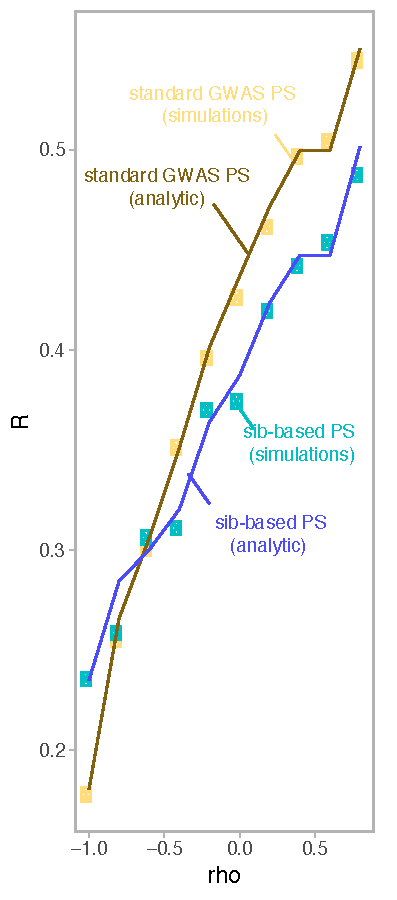
\includegraphics{supp_figures/R_vs_rho_indirect_simulation_and_analytic.pdf}
\caption{\small [XXX details on simulation params]}
\label{fig_R_vs_rho_sims}
\end{figure}

%\subsection{Consequences of direct-indirect correlation and significance threshold}
%\hl{to be completed}
%
%To gain some intuition we first note that \hl{[discuss with derivatives assuming fixed contribution across sites, add plot]} if indirect effects are strongly positively correlated with direct effects then prediction accuracy would be higher for standard GWAS than sib-regression.
%
%We next look at the effect of changing the significance threshold on SNPs (in the ascertainment set) that we include in our standard and sib-based polygenic scores.  We can rewrite eq.~\ref{R_indirect_general_form} as follows
%$$R=\frac{\sum_i^mA(i)}{\sqrt{\sum_i^mB(i)}},$$
%with
%$$A(i):=Var[x_i](\beta_i+\eta_i)E[\hat{\beta}_i]$$
%and
%$$B(i)=Var[y]Var[\hat{\beta}_i]E[x_i^2]+\sum_i^mVar[x_i]E[\hat{\beta}_i]^2$$
%being positive. We will approximate the effect of changing the p-value threshold as a change to the number of SNPs in the polygenic score ($m$).  The change in prediction accuracy as we change $m$ is
%$$\frac{dR}{\partial	m}=\frac{A(m)\sum_i^mB(i)+B(m)\sum_i^mA(i)}{(\sum_i^mB(i))^{\frac{3}{2}}}=(\frac{A(m)}{\sum_i^mA(i)}+\frac{B(m)}{\sum_i^mB(i)})R$$

% we fix $Var[x_i]$, $\beta_i$ and $\eta_i$ across all sites $i$, then $R^{ur}-R^{sib}$ is monotonically increasing with $\eta_i$.  This suggests to us that indirect effects that are positively correlated with direct effects give higher prediction accuracy for standard GWAS than sib-regression.  This also suggests that in the case of indirect effects tending to have the opposite sign, $R$ may even be negative for sib regression.
%\cite{Bischoff2006}
\pagebreak

\bibliographystyle{acm}

%\bibliography{sample_size_matching}

\end{document}

